\section{Contextual Dynamics}
\label{sec:condy}



The structure of our stepper is shown in Figure \ref{fig:structure}. We use the similar structure developed by \citet{cong_implementing_nodate}. The expression is first decomposed into many independent evaluation contexts. Then, user may choose one of them to step. And the stepper will compose them into final result. For example, in Figure \ref{fig:multiple}, we have 3 evaluation contexts highlighted as green boxes. And when we click the third one, only the expression in third box is evaluated and then composed into the whole expression.

\begin{figure}[htbp]
  \centering
  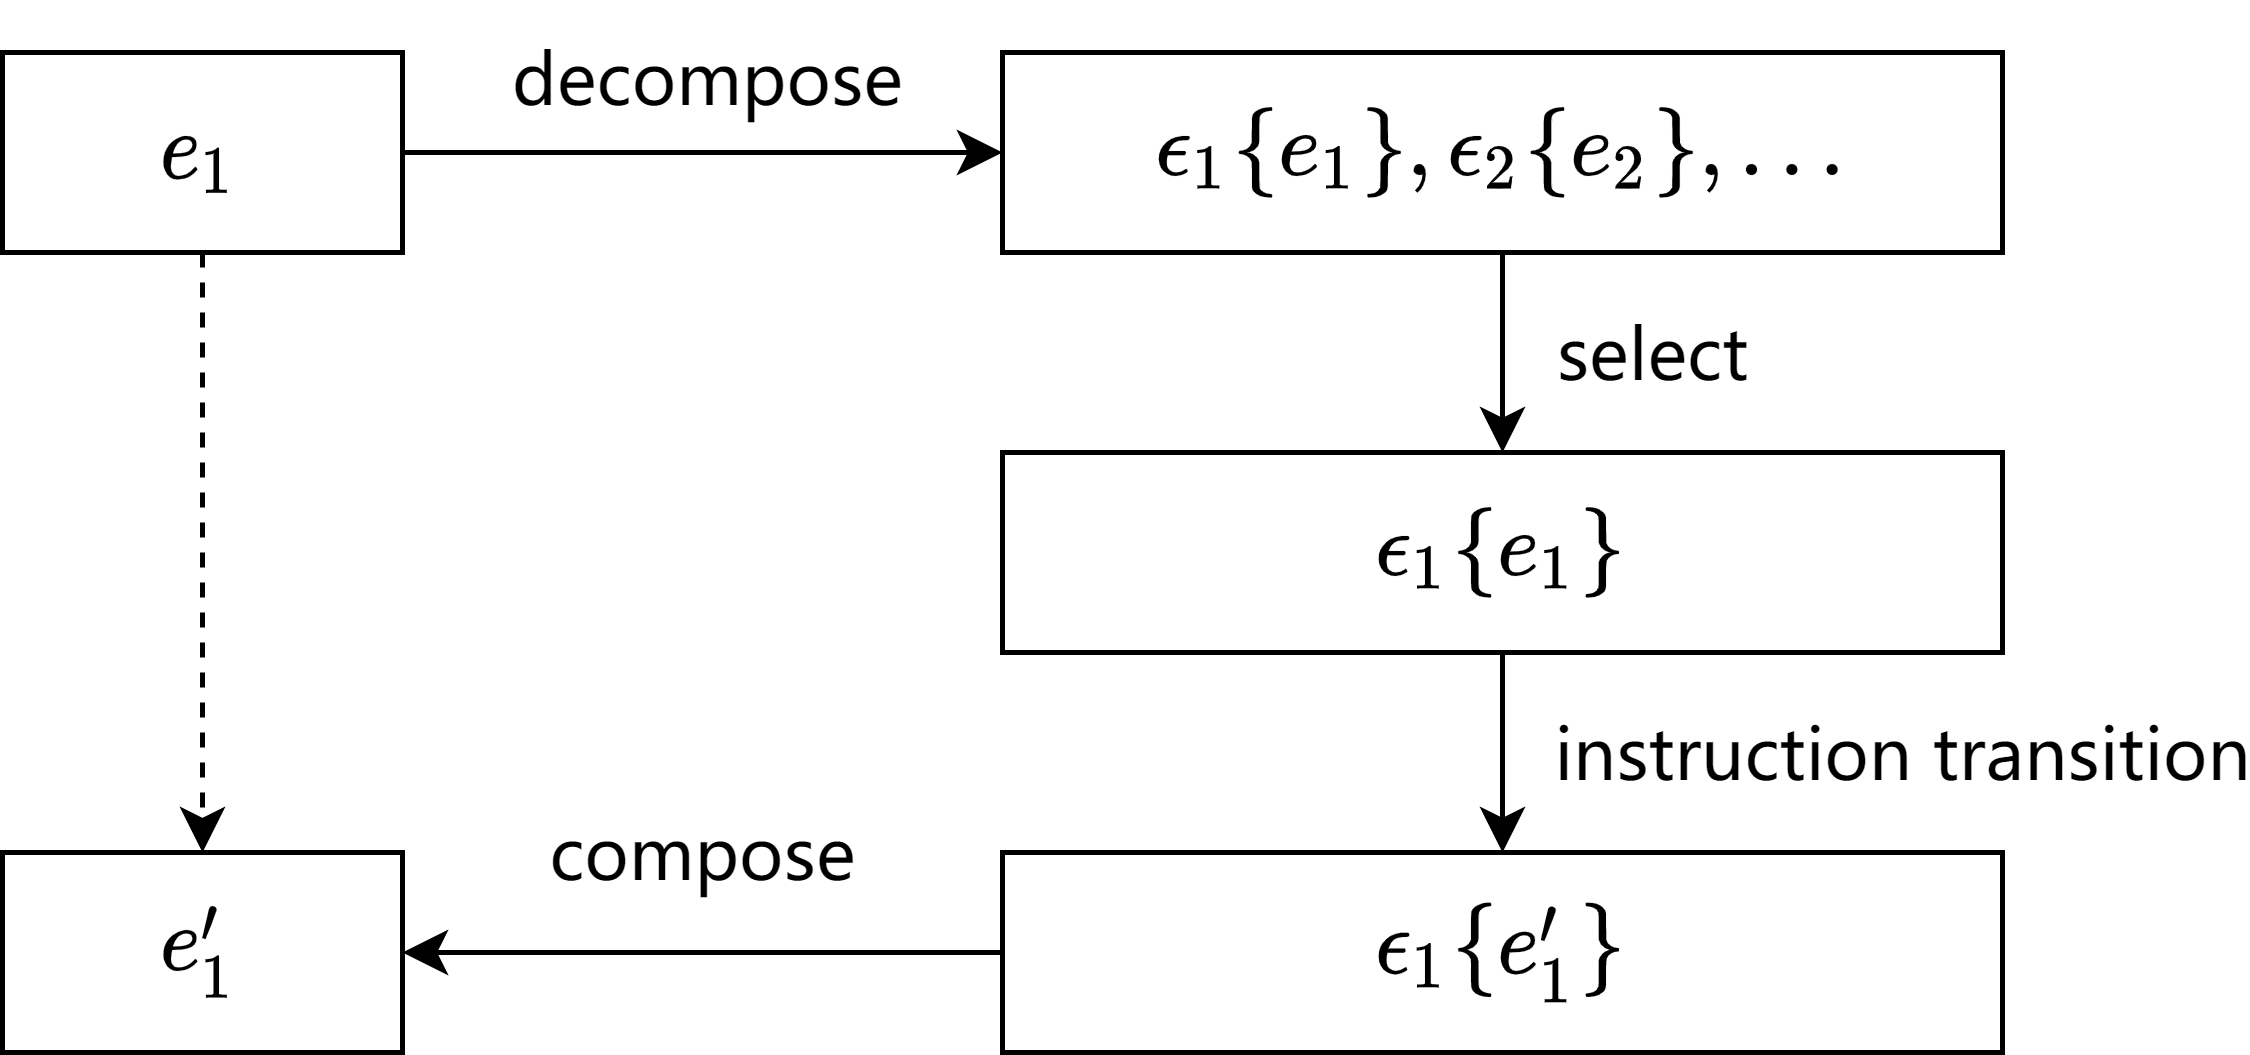
\includegraphics[width=0.5\textwidth]{img/struct.png}
  \caption{Structure of stepper}
  \label{fig:structure}
\end{figure}

We now formally define the instruction transition judgement denoted as $\htrans{e_1}{e_2}$. Figure \ref{fig:decompose} shows some of the transition judgements. Then, we have the formal definition of evaluation context. We show some of rules in Figure \ref{fig:decompose}. For any expression, we define the decompose function $\mathtt{decompose}(e)$ which returns all evaluation contexts of $e$. The formal definition is given below:
$$ \mathtt{decompose}(e) = \{ \epsilon\{e'\} | e = \epsilon\{e'\} \text{ and not } e' \mathtt{final} \}. $$

Unlike the regular evaluation context, this decompose function $\mathtt{decompose}$ will return a list of contexts that are steppable. So, there is a condition that $e'$ is not final. In general, we can see that if $\isFinal{e}$, $\mathtt{decompose}(e) = \emptyset$. We use addition as an example of non-final expressions. For expression $e_1 + e_2$, if both of them are final, we have $\mathtt{decompose}(e_1 + e_2) = \{ \hcontext{\circ}{e_1+e_2} \}$. Otherwise, 


\begin{align*}
  \mathtt{decompose}(e_1 + e_2) &= \{ \hcontext{(\epsilon_1 + e_2)}{e_1'} | \hcontext{\epsilon_1}{e_1'} \in \mathtt{decompose}(e_1)\} \\
  &\cup \{ \hcontext{(e_1 + \epsilon_2)}{e_2'} | \hcontext{\epsilon_2}{e_2'} \in \mathtt{decompose}(e_2)\}.
\end{align*}


\begin{figure}[htbp]
  \vspace{-3px} 
  \fbox{ $\htrans{e}{e'} $}~~\text{$e$ takes an instruction transition to $e'$}\hfill
  \begin{subequations}
  \label{eqns:instr_trans}
    \begin{mathpar}
        %\hfill
        \inferrule[]{\isFinal{e_2}
            }{
              \htrans{\hap{\lamfunc{x}{e_1}}{e_2}}{[e_2/x]e_1}
            }
        %\hfill
    \end{mathpar}
  \end{subequations}

$\arraycolsep=4pt\begin{array}{lll}
\text{EvalCtx}~~ \epsilon & ::= &
  \circ  ~\vert~
  \hap{\epsilon}{e} ~\vert~
  \hap{e}{\epsilon} ~\vert~
  \hhole{\epsilon} ~\vert~
  \epsilon + e ~\vert~
  e + \epsilon
\end{array}$

\fbox{ $e = \hcontext{\epsilon}{e'}$}~~\text{$e$ is obtained by replacing the mark in $\epsilon$ with $e'$}\hfill
  \begin{subequations}\label{eqns:decompose}
  \begin{mathpar}
      \hfill
      \inferrule[FHOuter]{
          }{
            e = \hcontext{\circ}{e}
          }\hfill
      \inferrule[FHAp1]{e_1 = \hcontext{\epsilon_1}{e_1'}}{\hap{e_1}{e_2} = \hcontext{\hap{\epsilon_1}{e_2}}{e_1'}}\hfill
      \inferrule[FHAp2]{e_2 = \hcontext{\epsilon_2}{e_2'}}{\hap{e_1}{e_2} = \hcontext{\hap{e_1}{\epsilon_2}}{e_2'}}\hfill
      \hfill
  \end{mathpar}
\end{subequations}
\hrule
\caption{Insturction transition and decomposition}
  \label{fig:decompose}
  \vspace{-5px}
\end{figure}


For example, we have an expression $e_0 = 4 + 1 + (5 + 6)$. First, we know that $\hdecom{4 + 1}{[\hcontext{\circ}{4 + 1}]}$ and $\hdecom{5 + 6}{[\hcontext{\circ}{5 + 6}]}$. So, According to the definition, we have,
$$
\hdecom{4 + 1 + (5 + 6)}{[\hcontext{(\circ + (5 + 6))}{4 + 1}, \hcontext{(4 + 1 + \circ)}{5 + 6}]}.
$$
User may choose second one so that the stepper will first evaluate $5 + 6$ and put result into mark. Hence, we get $4 + 1+ 11$ finally.